The muon system has a more complex reconstruction geometry than the other subsystems. It requires navigation both towards and within chambers, while also handling inert material in components such as the magnet coils and support structures correctly. To handle this, a dedicated navigation model based upon a frustum and octree is used.

In this model, each chamber is enclosed in a bounding box, and these boxes are used to construct an octree, which is a tree that recursively divides three-dimensional space into eight octants until a specified depth is reached. The resulting structure organizes all chambers within a single “top box” encompassing all volumes. An illustration of an octree can be seen in Figure~\ref{fig:reco_acts_muon_octree}.
\begin{figure}[htp]
  \centering
  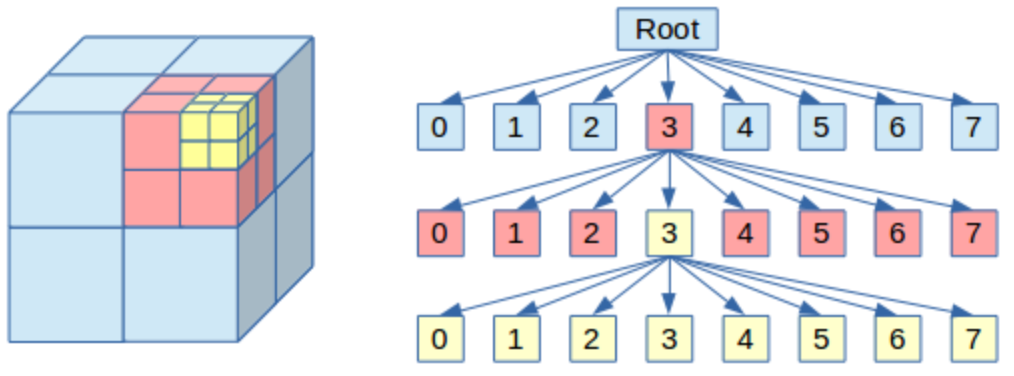
\includegraphics[width=0.8\textwidth]{figures/reco/reco_acts_muon_octree.png}
  \caption{An example of an octree with its subdivisions into octants. Taken from~\cite{geidav2014octrees}}\label{fig:reco_acts_muon_octree}
\end{figure}

For navigation, a frustum (see Figure~\ref{fig:reco_acts_frustum}) is built using the particle's position and direction. This frustum intersects the root node of the octree and descends through its children, identifying intersected bounding boxes. At the bottom level, the frustum yields a list of bounding boxes that have been intersected, and using those, a list of portal candidates are identified. An example of a frustum intersecting an octree can be seen in Figure~\ref{fig:reco_acts_frustum_octree}.

\begin{figure}[htp]
  \centering
  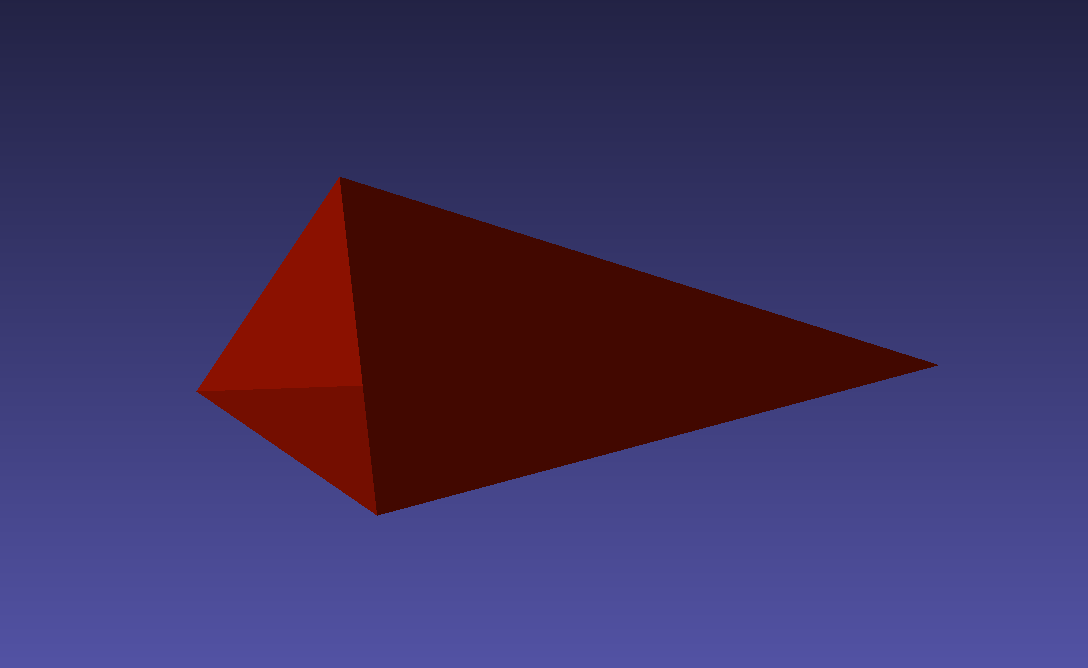
\includegraphics[width=0.8\textwidth]{figures/reco/reco_acts_frustum.png}
  \caption{An example frustum as seen in ACTS\@. It is essentially a cone-like object can more sides can be added.}\label{fig:reco_acts_frustum}
\end{figure}

If the particle exits the frustum during navigation, the frustum is recreated using the updated position and direction, and the octree is re-intersected to find new candidate portals. This approach ensures a fast lookup for portal candidates, allowing for efficient navigation between chambers.

Internally, a grid-based navigation model is used to handle the navigation within drift chambers. This model allows for efficient candidate surface lookup by mapping surfaces into a grid based on their position within the chamber. Once the grid is created, an artificial path through the chamber is constructed and the bins intersected in the grid are used to identify the candidate surfaces.

\begin{figure}[htp]
  \centering
  \subfloat[A frustum intersecting the root node]{
    \makebox[0.48\textwidth][c]{%
      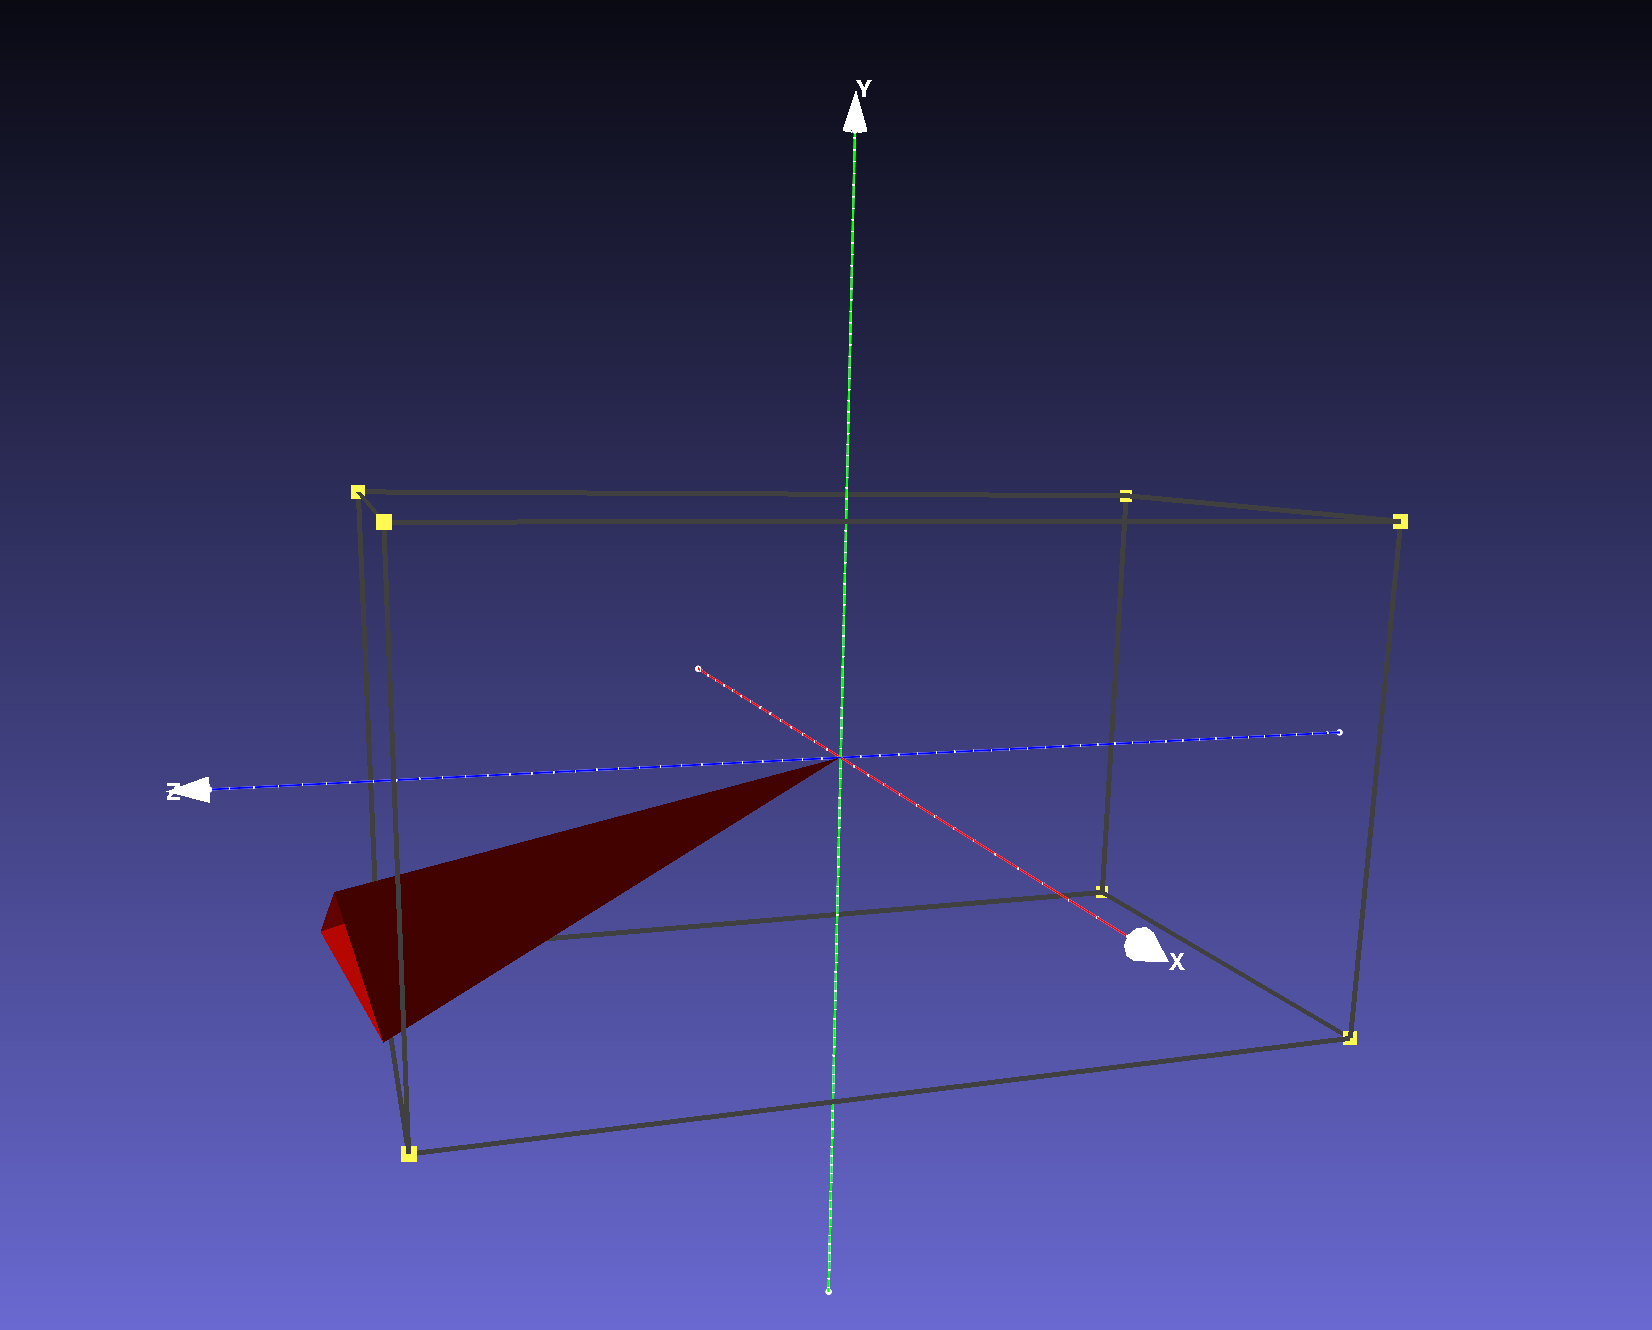
\includegraphics[height=0.4\textwidth,keepaspectratio]{figures/reco/reco_acts_frustum_intersect_root.png}%
    }\label{fig:reco_acts_frustum_intersect_root}
  }
  \hfill
  \subfloat[The volume candidates found by the frustum]{
    \makebox[0.48\textwidth][c]{%
      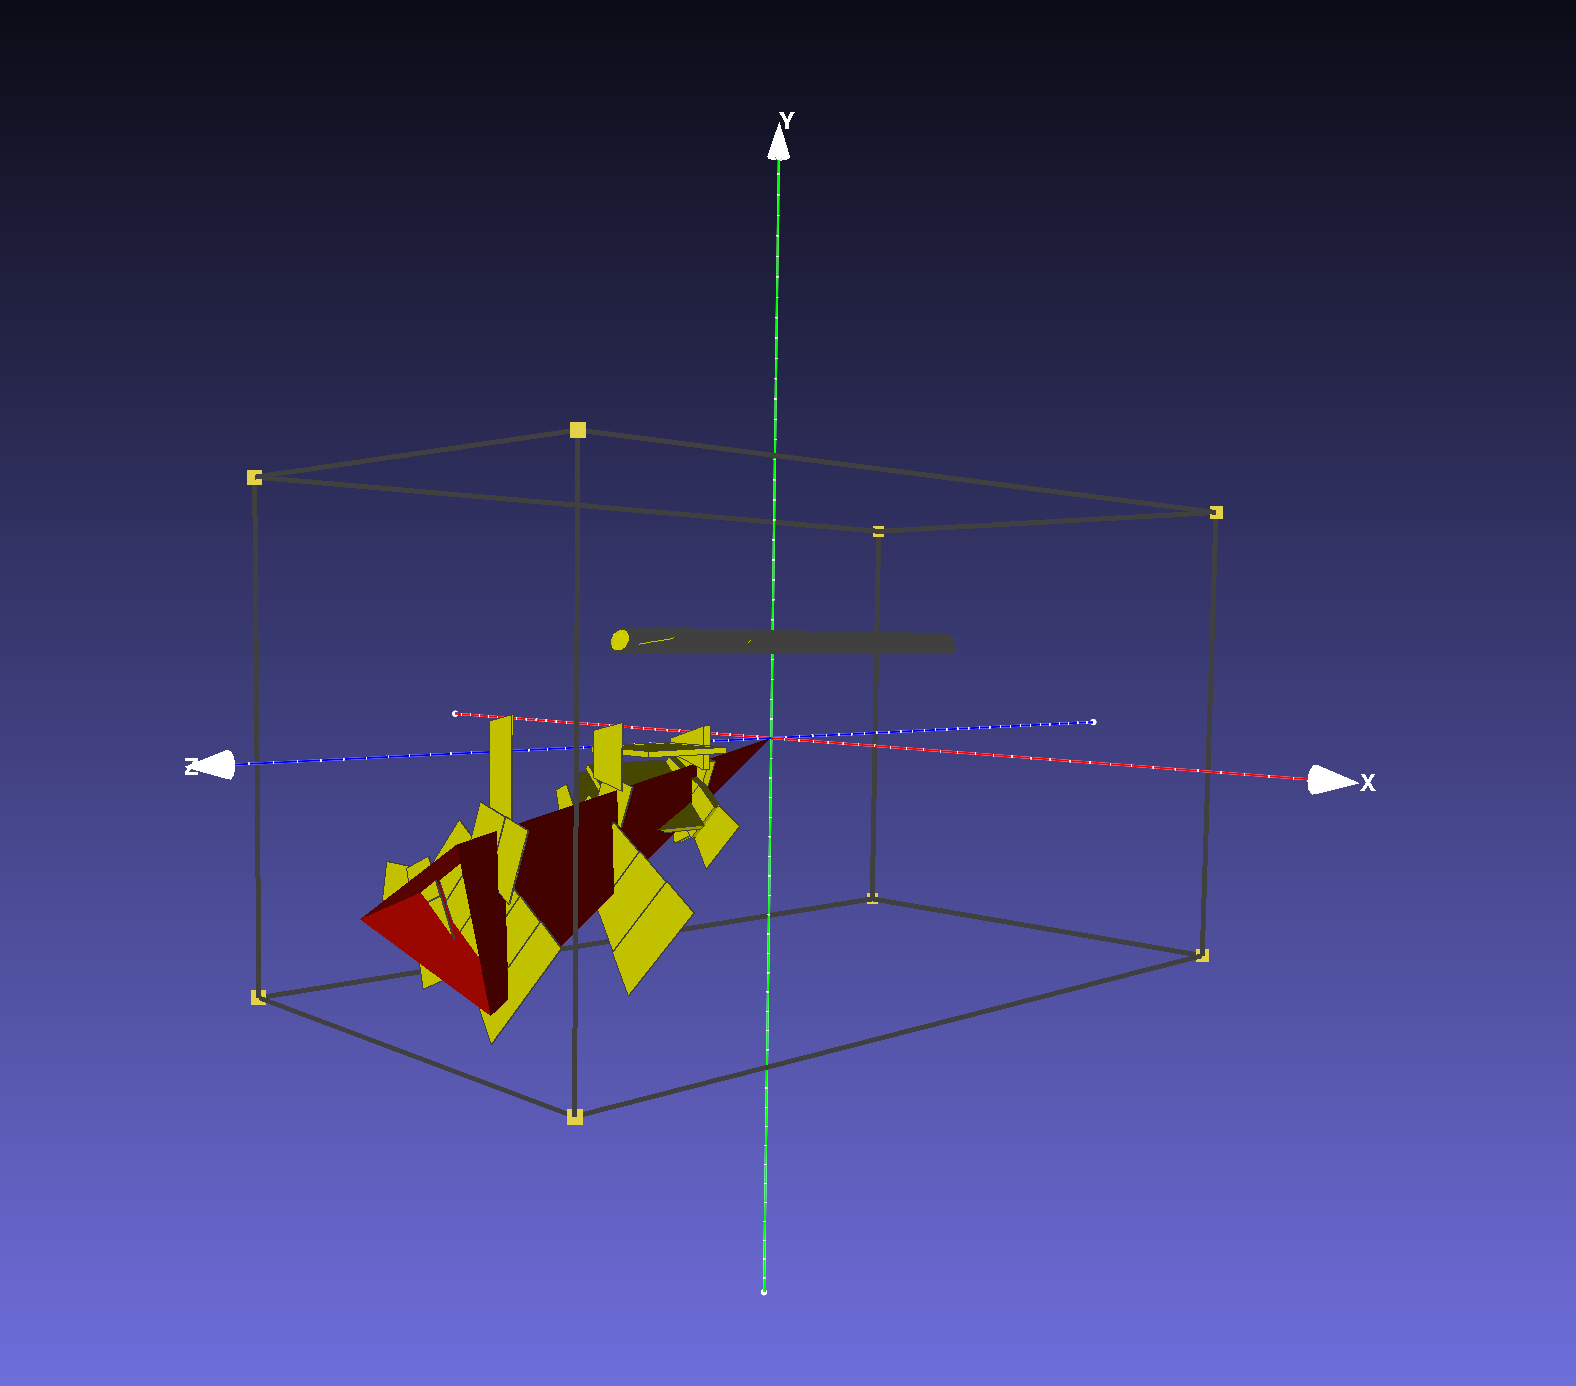
\includegraphics[height=0.4\textwidth,keepaspectratio]{figures/reco/reco_acts_frustum_finds_volume.png}%
    }\label{fig:reco_acts_frustum_finds_volume}
  }
  \caption{Left: An example of a frustum, shown in red, intersecting the root node, the outlined box. Right: The frustum, shown in red, with its found intersected volumes, in yellow.}
  \label{fig:reco_acts_frustum_octree}
\end{figure}
